% -----------------------------------------
% ------------ DON'T EDIT HERE ------------ 
% -----------------------------------------

\documentclass[11pt]{article}
\usepackage[a4paper, left=0.8in, right=0.8in, top=0.8in, bottom=0.8in, headheight=20pt]{geometry}
\usepackage{multirow}
\usepackage{array}
\usepackage[svgnames]{xcolor}
\usepackage{graphicx}
\usepackage{fancyhdr}
\usepackage{float}
\usepackage{hyperref}
\usepackage[final]{pdfpages}

\usepackage{transparent}
\usepackage{eso-pic}
\newcommand\BackgroundPic{%
\put(-240,0){%
\parbox[b][\paperheight]{\paperwidth}{%
\vfill
\centering
{\transparent{0.33} 
\centering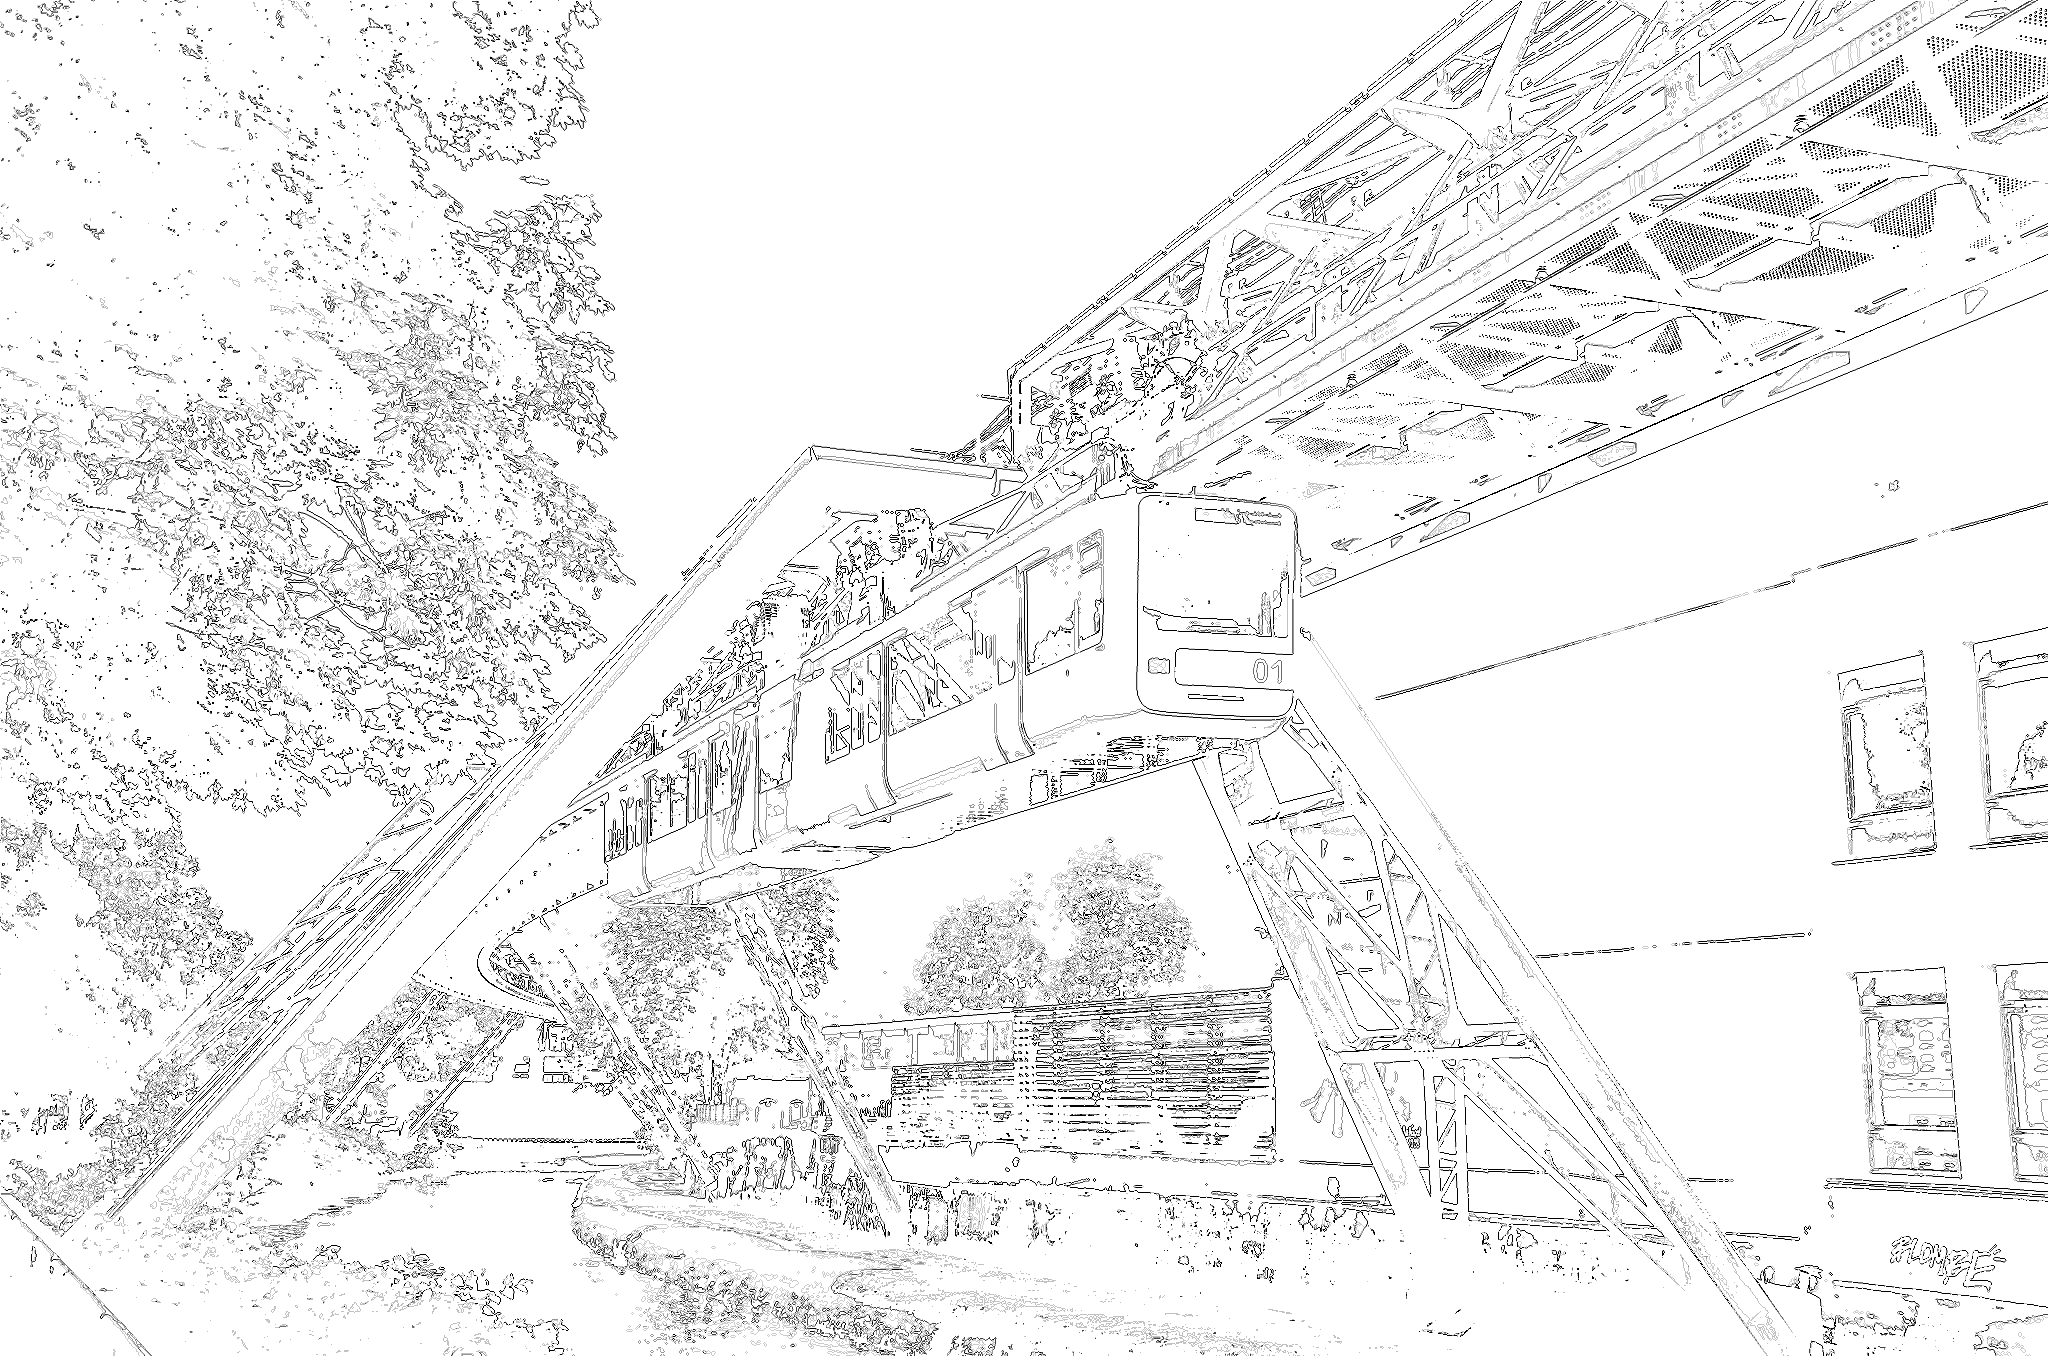
\includegraphics[height=\paperheight,%
keepaspectratio]{Figures-dontEdit/Schwebebahn_G15.png}}%
\vfill
}}}

\hypersetup{
    colorlinks=true,
    linkcolor=black,
    filecolor=black,      
    urlcolor=black,
    pdftitle={Overleaf Example},
    pdfpagemode=FullScreen,
    }

\definecolor{moderncvgreen}{rgb}{0.35,0.70,0.30}

\hypersetup{
colorlinks=true,
,citecolor=moderncvgreen
,citebordercolor=moderncvgreen
,urlbordercolor=moderncvgreen
}

\renewcommand*\contentsname{\textcolor{moderncvgreen}{\textsf{Table of Contents}}}


\newcolumntype{P}[1]{>{\raggedright\arraybackslash}p{#1}}


\pagestyle{fancy}
\fancyhf{}
\lhead{
\includegraphics[width=2.75cm]{Figures-dontEdit/wuppertal.png} \; \hspace{0.6cm}

\includegraphics[width=5cm]{Figures-dontEdit/izwt.jpg} \; \hspace{0.33cm} 
\includegraphics[width=5cm]{Figures-dontEdit/dfg_logo_schriftzug_blau_4c.eps}}
\rfoot{Page \thepage}


\usepackage[backend=biber, style=numeric-comp, sorting=none,uniquelist=false,natbib=true,doi=false,isbn=false,url=false,eprint=false,pagetracker, ibidtracker=constrict]{biblatex}
\addbibresource{references.bib}
\renewcommand*{\bibfont}{\normalfont\fontsize{8}{10}\selectfont}


\begin{document}

% \sffamily
\AddToShipoutPicture*{\BackgroundPic}
\thispagestyle{empty}

\vspace{2.5cm}

% \begin{figure}[H]
% \includegraphics[width=15cm]{Figures-dontEdit/SURF-V-RGB-BRush.png}
% \centering
% \end{figure}

\begin{flushright}
\textcolor{black}{
\textbf{
\Huge{
Methodological transformations \\ in fundamental physics}}
}
\end{flushright}

\begin{flushright}
\textbf{
\Large{
\textcolor{black}{
September 16th -- 18th 2024}}\\
\textcolor{black}{Wuppertal}}
\end{flushright}

\vfill 
\begin{flushright}
\color{moderncvgreen}
\textbf{
\Huge{
Workshop program}}
\end{flushright}

\begin{flushright}
\large{
\textcolor{black}{
\textbf{Organizing Committee}\\
Sarwar Ahmed\\
Lucas Gautheron\\
Anastasiia Lazutkina\\
Radin Dardashti}
}
\end{flushright}

\begin{flushright}
\textcolor{black}{
\textit{With help from Daniela Ebeling, Minori Nohara, 
Julian Heidinger, XXX}
}
\end{flushright}

\vspace{-0.5cm}

\newpage

\

\normalsize
\vspace{-1em}
The success of science is often attributed to “the” scientific method, yet the definition and nature of this method remains a subject of philosophical debate. While traditional philosophy sought to establish a normative, static and universal account of the scientific method (Carnap 1928; Popper 1959; Hempel 1966), more practice-oriented philosophers have stressed the dynamic nature of scientific method(s) since the post-positivist turn in philosophy of science (Kuhn 1962; Lakatos 1970; Laudan 1978; Nickles 1987; Humphreys 2004; Dawid 2013). This movement has culminated with radical stances such as  methodological anarchism (Feyerabend, 1975).

Recent developments in fundamental physics (string theory, the standard model of particle physics and its extensions, early universe cosmology, etc.) offer promising case studies for investigating (the) scientific “method(s)” and its alleged dynamic and plastic nature. This workshop therefore proposes to review recent developments in fundamental physics, in order to evaluate whether these developments entail significant methodological breaks with respect to the past. ``Methods'' is to be understood in a broad sense, including criteria of epistemic appraisal (acceptance) and heuristic appraisal (pursuit), and more globally the computational, observational, experimental, and statistical means through which evidence is produced and assessed. The workshop brings together perspectives from philosophers of science and physics, historians, physicists and social epistemologists.

\normalsize

\vfill

\tableofcontents

\newpage 

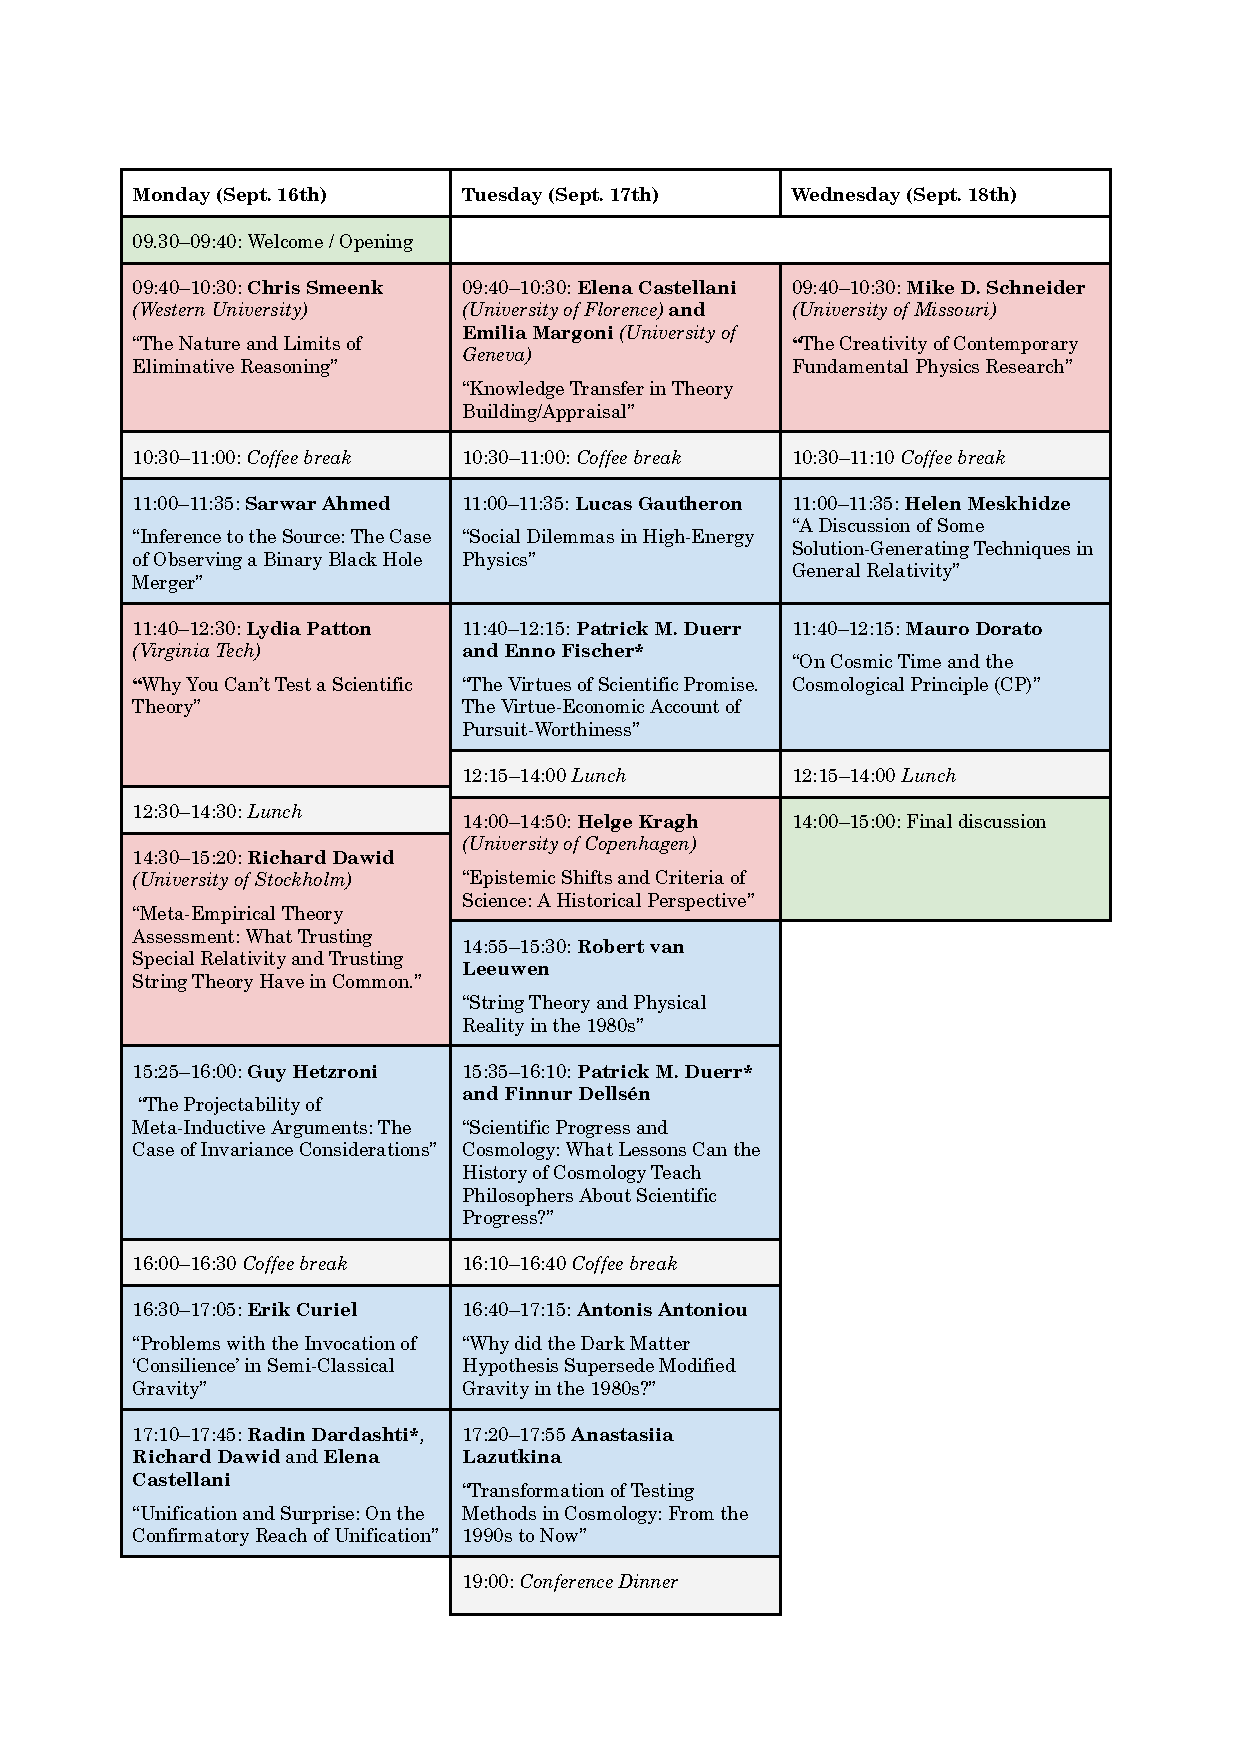
\includepdf[pages=1]{program.pdf}


\newpage


\section*{\textsf{Day 1 (Monday, September 16th)}}
\addcontentsline{toc}{section}{Day 1}
\vspace{3em}

% \subsection*{\textsf{\textcolor{Goldenrod}{SESSION A: Empirical and meta-empirical components of epistemic appraisal}}}
% \addcontentsline{toc}{subsection}{SESSION A: Symposium Theme TBD}

\subsection*{\textsf{``The Nature and Limits of
Eliminative Reasoning''}}
\addcontentsline{toc}{subsection}{``The Nature and Limits of
Eliminative Reasoning'' (\textbf{Chris Smeenk})}

\textcolor{moderncvgreen}{
\textit{Chris Smeenk, Western University
}
}

\ 

Eliminative reasoning is an appealing way to establish a theory: observations rule out all the competitors, leaving one theory standing. There have been long-standing debates in philosophy regarding the upshot and limitations of eliminative arguments.  The pattern of reasoning only works if we have taken all the viable alternatives into account; how can we have confidence that the correct theory is among the candidates surveyed? In this talk, I will defend the virtues and clarify the limitations of eliminative reasoning, based on seeing how it has been used in gravitational physics.  I will consider one case study of eliminative reasoning in detail, namely efforts to show that general relativity (GR) provides the best theory of gravity in different regimes.  Physicists have constructed parametrized spaces meant to represent a wide range of possible theories, sharing some core set of common features that are similar to GR.  I draw three main points from this case study.  First, the construction of a broad space of parametrized alternatives partially counters the ``problem of unconceived alternatives'' (due to Duhem and Stanford).  Second, this response is only partially successful because the eliminative arguments have to be considered in the context of a specific regime.  Solar system tests of gravity, using the PPN framework, favour GR — or any competing theories that are equivalent to it within this regime.  But, third, eliminative arguments in different regimes may be complementary, if theories that are equivalent in one regime can be distinguished in other regimes. These three points support a qualified defense of the value of eliminative reasoning, and further suggest a refinement of what is in fact supported by this kind of argument.

\

\newrefsection
\subsection*{\textsf{``Inference to the Source: The Case
of Observing a Binary Black Hole
Merger''}}
\addcontentsline{toc}{subsection}{``Inference to the Source: The Case
of Observing a Binary Black Hole
Merger'' (\textbf{Sarwar Ahmed})}

\textcolor{moderncvgreen}{
\textit{Sarwar Ahmed, University of Wuppertal
}}

\ 

The philosophical literature is replete with the discussion of theory-laden observation and circularity with regard to the evidential role of observation in testing and confirming theories. However, only a few philosophers have situated this discussion within the process of observation itself, that is, theory ladenness and circularity with respect to inference to the source. It has been argued that in order to infer the source reliably, the theory of the source should not be involved in the process of observation \cite{Hacking1983-HACRAI-7, Kosso1988-KOSDOO} or, if it is, there should be an independent empirical access \cite{Franklin2002-FRASAD-2}.

A number of scientists and philosophers of science have raised concerns about the epistemic aspects of observing binary black hole mergers. Specifically, concerns have been raised about the theory/model ladenness of binary black hole observation and its evidential role in testing general relativity in this extreme gravitational regime \cite{PhysRevD.80.122003}, as well as the alleged circularity of the observation \cite{Elder2023-ELDBHC}.

 Given that the observation of binary black hole merger does not fulfill any of the normative conditions for the inference to the source suggested by the philosophical accounts, how can the alleged circularity be mitigated?
 
In this paper, I argue that concerns about circularity in binary black hole observation is a consequence of the H-D method, and that the epistemic threat, if any, comes not from the theory-laden process, since modern observations are inherently theory laden, but from the underdetermination of the source by the collected data, since the data could be explained by proposing inconsistent sources for the gravitational waves. To reliably infer the source is to overcome this underdetermination.

I will further argue that a bidirectional version of inference to the only explanation captures the situation well and mitigates concerns about the inaccuracy of the models with respect to GR. However, to provide a full epistemic justification for the observation regarding the viability of GR as a background theoretical framework and its accurate description of the source system, one needs a broader conception of evidence to overcome the underdetermination. To this end, I will argue that the integration of meta-empirical assessments developed by Dawid \cite{Dawid2018-DAWDTU} into the inference to the only explanation is a promising strategy as a justifiable extension of the concept of evidence.

\printbibliography[heading=none]

\

\subsection*{\textsf{``Why You Can’t Test a Scientific
Theory''}}
\addcontentsline{toc}{subsection}{``Why You Can’t Test a Scientific
Theory'' (\textbf{Lydia Patton})}

\textcolor{moderncvgreen}{
\textit{Lydia Patton, Virginia Tech
}
}

\ 

The claim that you can’t test a scientific theory may seem audacious, since Karl Popper famously argued that only scientific theories can be falsified by evidence.  But strictly speaking, a purely theoretical framework has no intrinsic connection to observation - and conversely, observation has no intrinsic bearing on theoretical claims. Testing requires finding rigorous connections between speculative claims and experimental evidence, connections that are not given without work. In the case of gravitational wave astronomy, those connections have been built up over time in a way that mirrors Kevin Elliott’s methodological iteration: ``a process by which scientists move back and forth between particular modes of research'' (2012). As Wilson (2017) has argued, ‘theory T thinking’ is a very imperfect tool to investigate this kind of iterative progress, and as Halvorson (2012) urges, thinking of theories as classes of models does not capture what is interesting about them. Working from examples including gravitational wave astronomy and fluid mechanics, I propose that we think of theories as incorporating modal, explanatory, and heuristic reasoning. The question arises: once we incorporate the apparatus necessary to test a theory, is it still a theory?

\ 

\subsection*{\textsf{``Meta-Empirical Theory
Assessment: What Trusting
Special Relativity and Trusting
String Theory Have in Common.''}}
\addcontentsline{toc}{subsection}{``Meta-Empirical Theory
Assessment: What Trusting
Special Relativity and Trusting
String Theory Have in Common.'' (\textbf{Richard Dawid})}

\textcolor{moderncvgreen}{
\textit{Richard Dawid, Stockholm University
}
}

\ 

The epistemic appraisal of theories that lack conclusive empirical testing of their core predictions is a pre-eminent issue in fundamental physics today. From string theory to cosmic inflation, from dark matter to supersymmetry, fundamental physics deals with influential concepts that have so far eluded conclusive empirical testing. Grappling with the epistemic appraisal in such contexts has led to some of the most contentious debates in contemporary science.  Meta-empirical assessment has been proposed as a mechanism that constitutes a rational core of the described epistemic appraisals. In this talk, I want to develop the broader conceptual framework of meta-empirical assessment: meta-empirical assessment provides the backbone for assessing the effectiveness of the scientific method in general. Most importantly, it provides the basis for connecting empirical confirmation to trust in a theory’s empirical implications. Contexts where empirical testing is still missing are, from this perspective, special cases where meta-empirical assessment works under unusual circumstances. It is the under-appreciation of meta-empirical assessment as a core element of empirical confirmation that has made it difficult for many philosophers of science and quite some physicists to acknowledge that there can be legitimate trust in scientific theories in the absence of empirical confirmation.

\ 

\subsection*{\textsf{``The Projectability of
Meta-Inductive Arguments: The
Case of Invariance Considerations''}}
\addcontentsline{toc}{subsection}{The Projectability of
Meta-Inductive Arguments: The
Case of Invariance Considerations'' (\textbf{Guy Hetzroni})}

\textcolor{moderncvgreen}{
\textit{Guy Hetzroni, The Open University of Israel
}
}

\ 

The presented research argues that naturalist philosophy of science, i.e. the aim to understand scientific process using epistemological standards extrapolated from science itself, puts constraints on which meta-inductive arguments should be considered projectable. The implications on theory construction, theory assessment, and on the philosophical discourse on meta-induction will be demonstrated through two interrelated case studies: invariance arguments in theories of modified gravity and gauge-symmetry breaking vs. gauge invariance in particle physics.

Meta-inductive argumentation is a suggested way of evaluating the epistemic status and pursuit-worthiness of proposed theories and research programs, based on the similarity of the theoretical methods they apply to theoretical methods that have led to empirically successful theories. Meta-induction, together with other suggested approaches to theory assessment in the absence of empirical input, has invoked controversy, reflecting on the compatibility of theoretical practices in certain approaches to fundamental physics with familiar empirical standards  of science (see, e.g., Dawid, 2013; Dardashti, Dawid and Thébault, 2019). The presented research suggests a refined approach toward these issues by aiming to distinguish between projectable and non-projectable meta-inductive arguments.  The analysis is by analogy to the discourse on scientific induction, in particular  in the context of suggested naturalist solutions (e.g. by Boyd, 1991) to Goodman’s new riddle of induction. The analogy would be used to suggest a naturalist account of meta-induction, in terms of a reflective inductive-like inference on the scientific process itself. A notion of projectability is required, as given theoretical methods can be described and classified in numerous ways. Like in the case of naturalist accounts of scientific induction, this notion should be based on scientific knowledge expressed in background theories. More specifically, it is argued that projectable meta-induction is based on a reconstruction of theoretical methods used in established theories, in a way that maximizes the weight of evidence and its direct theoretical representation. Thus, projectable meta-induction is based on similarity between patterns of inference and filling of explanatory gaps, rather than on similarity between theoretical or mathematical concepts.

The account would be demonstrated using two examples involving invariance argument: the construction of gauge theories of gravity, and gauge invariant approaches to particle physics (i.e., without spontaneous breaking of gauge symmetry, see, e.g. Berghofer et al., 2023). I will argue that in both cases it is possible to understand the relevant invariance arguments in the established theories in terms of extrapolation from local evidence.  This reveals ways in which certain theories (gauge-invariant approaches and theories that can be constructed using certain dynamical, rather than geometrical, considerations) are based on more projectable considerations than their rival theories. 

\ 

\newrefsection
\subsection*{\textsf{``Problems with the Invocation of
‘Consilience’ in Semi-Classical
Gravity''}}
\addcontentsline{toc}{subsection}{``Problems with the Invocation of
‘Consilience’ in Semi-Classical
Gravity'' (\textbf{Erik Curiel})}

\textcolor{moderncvgreen}{
\textit{Erik Curiel\textsuperscript{1,2,3} % Put Authors Here
\newline
\textsuperscript{1}University of Bonn; \textsuperscript{2}Harvard University; \textsuperscript{3}Quantum Information Structure of Spacetime Consortium
}
}

\ 

Semi-classical gravity (SCG), including black hole thermodynamics (BHT), is one of the most dynamic, influential, and lionized fields in contemporary fundamental theoretical physics. Indeed, BHT in particular, and results in SCG more generally, yield without a doubt the most widely accepted, most deeply trusted set of conclusions in theoretical physics in which GR and QFT work together in seemingly fruitful harmony, not to mention thermodynamics. This is especially remarkable when one reflects on the fact that we have absolutely no experimental or observational evidence for any of it. Indeed we do not have the remotest empirical access to the regimes where we expect such effects to appreciably manifest themselves. Whence then—on the basis of what evidence, what kind of evidence—comes the profound confidence almost all theoretical physicists and many philosophers have in the results of the field? This question becomes even more poignant in light of two facts: that almost all the most important results in the field depend essentially on the Hawking effect, viz., that black holes radiate like ordinary thermodynamical black bodies and subsequently “evaporate” \cite{Wald2001, Carlip2014}; and it is standard practice in the field today to take the Hawking effect as a real phenomenon that can itself provide evidential warrant for further theoretical claims. Carlip \cite{Carlip2014}, p. 2, is exemplary in giving voice to the most widely accepted reason why most physicists (and I think philosophers) accept the Hawking effect as real:
\begin{quote}
[T]he Hawking temperature... ha[s] been derived in so many independent ways, in different settings and with different assumptions, that it seems extraordinarily unlikely that [it is] not real.
\end{quote}

Consilience!—that most puissant of all epistemic tools \cite{Whewell1858}. Most physicists, when they consider the question of why one is warranted in having credence in Hawking radiation as a feature of the real world, invoke (albeit, almost always implicitly) this idea. Wallace \cite{Wallace2018, Wallace2019} is exemplary in this regard among philosophers, giving explicit voice to the claim. Whatever else may be the case, however, this cannot be traditional, standard consilience, in at least three ways:

\begin{enumerate}
    \item The different derivations are all purely theoretical, not deriving from nor constrained by any empirical input.
    \item This is not a case in which the same equations or relations or model, or values of quantities, are being derived for a given phenomenon based on different types of interactions among different types of physical systems, as in the classic case of Perrin’s derivation of Avogadro’s number \cite{Perrin1910, Smith2020}. This is rather a case in which different physical assumptions are made about the very same class of physical systems and interactions among them, and calculations and arguments run in very different mathematical and conceptual frameworks.
    \item The different forms of derivation—based on S-matrix calculations, or tunneling, or algebraic state-construction, or Cauchy-Schrödinger evolution, or analysis of the stress-energy tensor operator, or holographic arguments, or... —all lead to conclusions, different “pictures” of the Hawking mechanism, with varying physical interpretations not always straightforwardly consonant with each other, and sometimes in outright contradiction with each other \cite{Curiel2024}.
\end{enumerate}

If arguments of the considered form, therefore, are to be capable of providing epistemic warrant for Hawking radiation, they must exhibit or conform to a new kind of consilience—which must be articulated and defended—or at least a new form of evidential argumentation having some similarities to traditional consilience. And that must be articulated and defended. I discuss some possibilities for doing so, and why I think them all to be inadequate for the desired result in the absence of constraint by empirical data.

\ 

\printbibliography[heading=none]

\

\subsection*{\textsf{``Unification and Surprise: On the
Confirmatory Reach of Unification''}}
\addcontentsline{toc}{subsection}{``Unification and Surprise: On the
Confirmatory Reach of Unification'' (\textbf{Radin Dardashti} et al.)}

\textcolor{moderncvgreen}{
\textit{Radin Dardashti\textsuperscript{1}, Richard Dawid\textsuperscript{2}, Elena Castellani\textsuperscript{3} % Put Authors Here
\newline
\textsuperscript{1}University of Wuppertal; \textsuperscript{2}Stockholm University; \textsuperscript{3}University of Florence
}
}

\ 

TBA


\newpage 

\section*{\textsf{Day 2 (Tuesday, September 17th)}}
\addcontentsline{toc}{section}{Day 2}
\vspace{3em}

\subsection*{\textsf{``Knowledge Transfer in Theory
Building/Appraisal''}}
\addcontentsline{toc}{subsection}{``Knowledge Transfer in Theory
Building/Appraisal'' (\textbf{Elena Castellani, Emilia Margoni})}

\textcolor{moderncvgreen}{
\textit{Elena Castellani\textsuperscript{1},Emilia Margoni\textsuperscript{2},  % Put Authors Here
\newline
\textsuperscript{1}University of Florence; \textsuperscript{2}University of Geneva
}
}

\ 

Knowledge transfer, a phenomenon widely analyzed within several research areas, regards
the circulation and rearrangement of ideas, models, methodologies, as well as domain-specific
practices and protocols within different fields of inquiry. Recently, there has been a renewal of
interest in the nature and methodology of such transfer processes, their applicative potential
as well as their limitations. Within the context of this endeavor, we address the import of
knowledge transfer from the standpoint of theory building and appraisal. Our primary focus
will be the birth and development of the renormalization group as a particularly instructive
cross-fertilization process between quantum field theory, statistical mechanics and condensed
matter physics. On this, we propose a novel concept, which we christen cluster transfer, as
more apt for addressing the dissemination of the renormalization group framework. We then
go on to show the relevance of such a concept to capture the development of the flourishing
field of quantum gravity, and more generally for the evaluation of pursuitworthiness in fundamental physics programs.

\ 

\newrefsection
\subsection*{\textsf{``Social Dilemmas in High-Energy
Physics''}}
\addcontentsline{toc}{subsection}{``Social Dilemmas in High-Energy
Physics'' (\textbf{Lucas Gautheron})}
\textcolor{moderncvgreen}{
\textit{Lucas Gautheron\textsuperscript{1,2},
\newline\textsuperscript{1}University of Wuppertal; \textsuperscript{2}École Normale Supérieure
}
}

\

We all have heard the truism that ``physics is a social construct'', and it seems that everything has been said about it in the course of the ``Science Wars'' that opposed realists to constructivists. Yet, there is more to it! In this talk, I will contend that the (obvious) fact physics is a collective enterprise has meaningful consequences for scientific methodology, and raises interesting \textit{normative} issues for high-energy physics in particular.

I will begin by reviewing results from social epistemology: a) the ``independence thesis'', according to which learning strategies that are optimal for isolated individuals may fail for groups \cite{MayoWilson2011}, and b) impossibility results in judgment aggregation, which highlight the difficulty of dealing with disagreement in scientific collaborations \cite{list2002aggregating,Marcoci2020}. From a normative standpoint, these are legitimate issues for scientific methodology, given that there are ``worse'' and ``better'' ways of dealing with them.

I will then propose an alternative approach to the matter, by looking into various epistemically consequential social dilemmas that arise in the course of scientific inquiry, in particular in high-energy physics. Dilemmas involve a choice between alternatives that each present some disadvantage, thus prompting individuals to navigate a trade-off between different objectives. I will explore three examples of such trade-offs arising in high-energy physics. In each case, I will appeal to computational methods, and insights from social epistemology and cultural evolution.

The first dilemma involves the balance between \textit{independent} and \textit{cooperative} learning.  While cooperative learning is faster and enables more complex solutions, it introduces coordination costs and is more likely to miss globally optimal solutions \cite{Smaldino2023,Zollman2009}. This is not just a social epistemologist's fantasy: it is for instance a reality at the Large Hadron Collider, where the ATLAS and CMS experiments are individually cooperative (involving thousands of collaborators each), and yet seek to maximize their independence.

The second dilemma involves the balance between the variety of epistemic domains that we allow ourselves to explore (\textit{diversity}), and the requirement that we can exchange knowledge across these very domains (\textit{integration}) \cite{Schimmelpfennig2021}. I will demonstrate the tension with the example of supersymmetry: once thought to illuminate both the pursuit of quantum gravity and the physics of the electroweak sector, prospects of finding evidence for it in colliders are now looking very grim. We have legitimate epistemic reasons for \textit{not} requiring that physical theories such as supersymmetry improve our knowledge of certain epistemic domains like the electroweak sector, if it allows for progress in other epistemic domains (e.g. quantum gravity). However, this means that exchanges of knowledge among physicists will be limited: we have traded-off diversity for integration \cite{Gautheron2023}.

The third dilemma involves the balance between the need for scientists to fully take advantage of their prior knowledge (\textit{exploitation}), and the need to adapt to new evidence and opportunities (\textit{adaptation}). Using a mathematical framework called ``Optimal Transport'', I will demonstrate that high-energy physicists have been collectively adapting to changes in their epistemic landscape over the years 2000--2020 in a way that minimizes learning costs \cite{Gautheron2023a}. This shows that strategies of gradual adaptation efficiently address this trade-off, and suggests that the maximization of the utility of scientific capital accumulated in various forms (explicit/tacit knowledge, or material infrastructure) is a significant component of scientific rationality in high-energy physics.

\

\printbibliography[heading=none]

\

\subsection*{\textsf{``The Virtues of Scientific Promise.
The Virtue-Economic Account of
Pursuit-Worthiness''}}
\addcontentsline{toc}{subsection}{``The Virtues of Scientific Promise.
The Virtue-Economic Account of
Pursuit-Worthiness'' (\textbf{Patrick M. Duerr
and Enno Fischer}*)}

\textcolor{moderncvgreen}{
\textit{Patrick M. Duerr\textsuperscript{1},Enno Fischer\textsuperscript{2},  % Put Authors Here
\newline
\textsuperscript{1}University of Tübingen; \textsuperscript{2}Dresden University of Technology
}
}

\

When should we regard a scientific hypothesis as sufficiently promising to merit pursuit? That is, what
are the criteria for deciding whether it’s rationally justified to further work on an auspicious hypothesis
(e.g. by elaborating its foundations, applying it to new domains, or subjecting it to tests)? These
questions are particularly pressing for fledgling hypotheses whose evidential-epistemic status is still
inconclusive, as common at the forefront of contemporary fundamental physics (e.g., quantum gravity
scenarios or Beyond the Standard Model particle physics). Drawing on ideas by Peirce and Kuhn, this
presentation will elaborate and defend what we call the virtue-economic account of pursuit-worthiness.
Our approach appraises a hypothesis’ pursuit-worthiness in terms of a cognitive cost/benefit analysis.
Here, we take the cognitive benefits in question to consist in the hypothesis’ likely potential to instantiate
theory virtues (such as predictive power, explanatory power, unificatory power, coherence, fertility, etc.);
the costs correspond to the research efforts that one is likely to have to invest. Again, theory virtues
(simplicity and heuristic power in particular), as well as their absence (or even theory vices) are key
determinants of such costs. One task of the talk is to flesh out the details of the virtue-economic account.
In particular, we’ll clarify whom we take to be the relevant decision-maker: the researcher qua ideal
representative of the pertinent scientific (sub-)community.
The other task of the talk is to highlight the merits of this approach to pursuit-worthiness. First, with its
combination of subjective and objective elements—both in the interpretation and weighting of
individual theory virtues—it allows for exactly the flexibility in individual choices between consensus-
oriented conservativism and dissensus-tolerant speculation that an intellectually healthy dynamics of
science requires for the exploration of bold new ideas.
Secondly, the model’s normative dimension—its prescriptive assertion that auspicious hypotheses in the
above sense ought to be further pursued—follow naturally from standard decision-theoretical
assumptions: pursuit-worthiness, as our model spells it out, is an instance of garden-variety instrumental
rationality given the aims of science, and the stock of knowledge of the relevant scientific community.
Thirdly, our model is, we claim, descriptively adequate. Not only does it do justice to variety of reasons
for pursuit (e.g. from toy theories and explorative research to whittling down the range of serious
candidates to subject them to, say, eliminative induction), and naturally accommodates also a broad
spectrum of pursuit-worthy ideas (e.g. spanning concrete theories, new formalisms and interpretations,
anomalies, and experiments). The approach is also a fertile tool for illuminating the rational dynamics
behind major episodes in the history of physics, such as the Steady State controversy, the emergence of
the inflationary paradigm in primordial cosmology. It’s also apt to shed light on pressing present-day
quandaries, such as the status of SuSy or the Dark Matter/Energy conundrum.
Finally, we’ll demarcate our model from other extant proposals for pursuit-worthiness (such as Kuhn’s,
Laudan’s, Achinstein’s, Šešelja \& Straßer’s, and DiMarco \& Khalifa’s). The former, we submit, has various
advantages over the latter.

\

\subsection*{\textsf{``Epistemic Shifts and Criteria of
Science: A Historical Perspective''}}
\addcontentsline{toc}{subsection}{``Epistemic Shifts and Criteria of
Science: A Historical Perspective'' (\textbf{Helge Kragh})}

\textcolor{moderncvgreen}{
\textit{Helge Kragh, University of Copenhagen
}
}

\

In part inspired by the emergence of radically new theories of physics and
cosmology (e.g., string theory, the multiverse, pre-big-bang scenarios), during the
last couple of decades, physicists and philosophers of science have discussed – once
again – the fundamental question of what science is and what it is not. Does science
need to be redefined? The raison d’être for much of the current discussion seems to
be a feeling in some corners of the scientific community that modern fundamental
physics is in a state of crisis that necessitates a reconsideration of traditional
methodological criteria. Among these criteria, the most important is undoubtedly
the broadly accepted view that a theory, to be scientific, must be empirically testable
and preferably falsifiable. Although there are other ways of evaluating a theory, the
actual possibility of experimental or observational tests is typically considered a sine
qua non for a theory being scientific. It is this traditional view which is currently
questioned not only by some philosophers but also by some scientists, mostly but
not only physicists.
The paper will briefly discuss different forms of testability and their relative merits
with special attention paid to Karl Popper’s philosophy of science and its role played
in the recent controversy over the multiverse. (I also intend so say something about
‘principles’ in modern and not-so-modern physics.) Both as regards testability and
other methodological issues turning up in the modern debate, I argue that a proper
historical perspective is crucially important. It is only by taking the history of science
seriously that one can evaluate how novel and important the recent claims of meta-
empirical criteria really are. Indeed, in view of the many and somewhat similar
methodological discussions that occurred in earlier science, those of the present era
may well appear less dramatic and far from exceptional. But, of course, one should
be cautious when appealing to historical analogies or otherwise using examples
from the history of science to illuminate the present situation and draw conclusions
from it. Yet, although history is admittedly of limited use as a guide to the future, it
is the only guide of some degree of reliability that we have. It seems to me that the
historical approach provides reasons for skepticism with regard to current
suggestions of epistemic shifts of such a drastic nature that they amount to a new
definition of science.
As mentioned, suggestions of major epistemic shifts have occurred repeatedly in
earlier science, both in physics and elsewhere. As I see it, there is no reason to stick
to post-World War II science as instructive discussions of this kind go all the way
back to Descartes and the birth of science as we know it today. Some of these
examples are of relevance to the modern discussion, such as the nineteenth-century
theory of vortex atoms, Eddington’s advocacy of non-empirical fundamental physics
from the 1930s, and the cosmological controversy during the 1950s between the
steady-state universe and evolutionary models based on general relativity.

\ 

\newrefsection
\subsection*{\textsf{``String Theory and Physical
Reality in the 1980s''}}
\addcontentsline{toc}{subsection}{``String Theory and Physical
Reality in the 1980s”'' (\textbf{Robert van Leeuwen})}

\textcolor{moderncvgreen}{
\textit{Robert van Leeuwen, University of Amsterdam
}
}

\

In this historical talk I will explore the multiple ways in which string theorists related their theory to physical reality when it was developed as a paradigmatic approach in fundamental high-energy physics in the mid-1980s. ‘Physical reality’ is to be understood in a broad sense here, including (among others) already available experimental data, new empirical predictions that potentially could be tested, accepted physical theory, and theoretical structure that physicists believed to be reflected in nature.

As a starting point, I take the three papers that form the basis for the establishment of the modern string program: ‘Anomaly Cancellation in Supersymmetric \( D = 10 \) Gauge Theory and Superstring Theory’ \cite{green1984anomaly}, ‘Vacuum Configurations for Superstrings’ \cite{candelas1985vacuum}, and ‘Heterotic String’ \cite{gross1985heterotic}. Among others, based on interviews with contributors, I will describe how various ‘empirical’ motivations, such as the presence of chiral fermions in the theory and bottom-up demands for ‘realistic physics’, motivated the theory’s acceptance and development.

In addition, I will explain how the establishment of string theory was embedded in long-term developments in theoretical particle physics that already played a role in the late 70s and early 80s. These include the construction of supergravity, the revival of Kaluza-Klein theory as an approach to unification, attempts to solve the hierarchy problem using supersymmetry breaking, and the issue of confinement in QCD.

Finally, I will sketch how in the late 1980s one can identify a split between a perturbative approach of string phenomenology, aiming to derive Standard Model physics from string theory, and an approach focused on further expanding string theory’s non-perturbative structure.

Taken together, I hope this talk will illuminate how string theorist’s ‘methods’ can be seen both as a continuation of the theoretical particle physics tradition from the 1970s, while at the same time thoroughly transformed this. When it comes to the role of empirical data in theory construction, the ambiguity in how string theorists considered their theory-in-progress to be connected to physical reality is of crucial importance in this development.

\textit{The talk is based upon a chapter-in-progress of the presenter’s PhD thesis.}

\ 

\printbibliography[heading=none]

%Literature
%Candelas, P., Horowitz, G. T., Strominger, A., & Witten, E. (1985). Vacuum configurations for
%superstrings. Nuclear Physics B, 258, 46–74. https://doi.org/10.1016/0550-
%3213(85)90602-9
%Green, M. B., & Schwarz, J. H. (1984). Anomaly cancellations in supersymmetric D = 10
%gauge theory and superstring theory. Physics Letters B, 149, 117–122.
%https://doi.org/10.1016/0370-2693(84)91565-X
%Gross, D. J., Harvey, J. A., Martinec, E., & Rohm, R. (1985). Heterotic string. Physical Review
%Letters, 54(6), 502–505. https://doi.org/10.1103/PhysRevLett.54.502

\

\subsection*{\textsf{``Scientific Progress and
Cosmology: What Lessons Can the
History of Cosmology Teach
Philosophers About Scientific
Progress?''}}
\addcontentsline{toc}{subsection}{``Scientific Progress and
Cosmology: What Lessons Can the
History of Cosmology Teach
Philosophers About Scientific
Progress?'' (\textbf{Patrick M. Duerr*
and Finnur Dellsén})}

\textcolor{moderncvgreen}{
\textit{Patrick M. Duerr\textsuperscript{1},Finnur Dellsén\textsuperscript{2},  % Put Authors Here
\newline
\textsuperscript{1}University of Tübingen; \textsuperscript{2}University of Iceland
}
}

\

This paper examines philosophical accounts of scientific progress through a consideration of the
history of modern cosmology from Einstein’s 1917 model of the cosmos to the present-day
standard model of cosmology. We focus, in particular, on the epistemic account, on which
progress consists in the accumulation of knowledge, and the noetic account, on which progress
is analysed in terms of improved understanding. From the historical development of cosmology,
which we take to be representative in many regards of a bona fide progressive scientific
discipline, we draw three main lessons for these accounts:


\begin{enumerate}
    \item It is often difficult to locate—to pinpoint the locus of—the precise epistemic content of
scientific theories, i.e. the parts of these theories that can be considered knowledge. In
these cases, progressive scientific theories display a form of epistemic holism that
prevents the sort of accumulation of knowledge that the epistemic account requires.
\item  In science, a variety of justificatory practices and modes of reasoning are often
employed. More often than not, they fall short of the fastidious epistemic standards of
the epistemic acccount.
\item  Often, progressive theories defy easy and unambiguous characterisation in terms of
truth (even approximate truth), or its surrogates such as truth-likeness (verisimilitude).

\end{enumerate}

We argue that these three lessons (1)-(3) pose significant challenges to the epistemic account
of scientific progress. By contrast, the noetic account, with its emphasis on explanatory and
predictive dependency relations, can naturally accommodate these lessons.

\

\subsection*{\textsf{``Why did the Dark Matter
Hypothesis Supersede Modified
Gravity in the 1980s?''}}
\addcontentsline{toc}{subsection}{``Why did the Dark Matter
Hypothesis Supersede Modified
Gravity in the 1980s?'' (\textbf{Antonis Antoniou})}

\textcolor{moderncvgreen}{
\textit{Antonis Antoniou, National and Kapodistrian University of Athens
}
}

\

Throughout the 1960s and 1970s a series of cosmological observations and theoretical developments
highlighted the presence of various anomalies at the galactic and cosmological scale. These anomalies
could, in principle, be explained by pursuing one of the following two working hypotheses, which
would eventually be incorporated into a more comprehensive scientific theory:

\begin{itemize}
    \item WH1: The postulation of dark matter, a massive non-baryonic field which interacts with baryonic matter mainly via gravity, or,
    \item WH2: The modification of standard Newtonian dynamics in the regime of low accelerations,
and consequently of the theory of general relativity of which this new gravity would be a limit
\end{itemize}

% \newline

% • WH1: 

% \newline


% • 

% \newline

The hypothesis of dark matter would later be integrated in the $\Lambda$CDM model, the standard
cosmological model about the universe that assumes the correctness of the theory of general relativity
and requires the existence of cold dark matter and dark energy. The hypothesis of modified gravity
was mainly embedded in various versions of Modified Newtonian Dynamics (MOND), a group of
effective theories of gravity in which standard Newtonian dynamics cease to obtain below a critical
acceleration constant. Today, despite the diligent efforts of the MOND community to develop a
coherent relativistic version of MOND, the overwhelming majority of the physics community favours
the $\Lambda$CDM model and is often dismissive of the merits of MOND and its relativistic extensions.
The aim of this article is to examine why in light of certain observations and theoretical developments
by the 1980s, the scientific community almost in its entirety opted to pursue the hypothesis of dark
matter as opposed to the hypothesis of modified gravity, regardless of the theory into which the latter
would eventually be embedded. A plausible answer to these questions is given in terms of (i) the
problem-solving potential, (ii) the compatibility, (iii) the feasibility of incorporation and (iv) the
independent testability of the two competing hypotheses. When considered jointly, these four criteria
make a compelling case for explaining the underlying reasons for the strong inclination of the scientific
community to pursue the incorporation of dark matter in the standard model for cosmology, as
opposed to the development of possible modifications in standard gravitational dynamics. A
comparison between the dark matter case and the dark energy case is also presented, explaining why
in the latter case, the hypothesis of modified gravity is still widely considered as a viable explanation
for dark energy phenomenology, as opposed to the dark matter case.

\

\subsection*{\textsf{``Transformation of Testing
Methods in Cosmology: From the
1990s to Now''}}
\addcontentsline{toc}{subsection}{``Transformation of Testing
Methods in Cosmology: From the
1990s to Now'' (\textbf{Anastasiia
Lazutkina})}

\textcolor{moderncvgreen}{
\textit{Anastasiia
Lazutkina, University of Wuppertal
}
}

\

TBA

\newpage 

\section*{\textsf{Day 3 (Wednesday, September 18th)}}
\addcontentsline{toc}{section}{Day 3}
\vspace{3em}

\subsection*{\textsf{``The Creativity of Contemporary
Fundamental Physics Research''}}
\addcontentsline{toc}{subsection}{``The Creativity of Contemporary
Fundamental Physics Research'' (\textbf{Mike D.~Schneider})}

\textcolor{moderncvgreen}{
\textit{Mike D.~Schneider, University of Missouri
}
}

\

Braneworlds, chameleons, fuzzballs,.... Fundamental physics research today is not only creative, but impressively so. I'd like to understand why. History, sociology, anthropology, and even psychology are all plausibly relevant, but it is ambiguous how to piece together the many different threads. Lately, I've been thinking a lot about what really is the underlying notion of "creativity" in play when we talk about the dynamics of science. And in that vein, I have developed an account of uncreativity, on the basis of which it seems reasonable to propose that we interpret creativity as overcoming uncreativity. In this talk, my aim is to introduce the account of uncreativity, motivate thinking about creativity as overcoming uncreativity (given the account), and then explore whether this perspective gives some resources to articulate a promising singular hypothesis about why fundamental physics research is so impressively creative. (I am optimistic that it does.) But a theoretical perspective only does so much. The empirical parts of science studies are ultimately how that hypothesis may acquire real substance, and are where it tests its mettle. 

\ 

\subsection*{\textsf{``A Discussion of Some
Solution-Generating Techniques in
General Relativity''}}
\addcontentsline{toc}{subsection}{``A Discussion of Some
Solution-Generating Techniques in
General Relativity'' (\textbf{Helen Meskhidze})}

\textcolor{moderncvgreen}{
\textit{Helen Meskhidze, Harvard University
}
}

\

One area of contemporary physics that is presenting novel methodological challenges is
generating novel analytic solutions to Einstein’s field equation (EFE). Generating novel solutions
is important for several reasons. First, the known analytic solutions describe highly idealized
circumstances, some of which are nonetheless useful (e.g., the FLRW spacetime) but many of
which are highly unphysical. Expanding the known solution space is thus an important goal.
Another reason is that even the useful analytic solutions—the ones we use to describe
observed astrophysical systems—have various issues. For instance, the Kerr solution used in
current models of black holes has known curvature singularities. Yet another reason is that
analytic solutions can be very useful for guiding numerical analysis techniques. Such techniques
are required to model more complex systems, e.g., binary black hole mergers. Benchmarking
them against known analytic solutions is an important aspect of their development/methodology.


However, EFE describes a coupled system of nonlinear, second order partial differential
equations, making it difficult to solve. There are a number of methods that are used to generate
new analytic solutions, often exploiting symmetries of the mathematical structures involved.
Amongst the methods used for generating solutions, one stands out for both its effectiveness
and its puzzling character: the Newman-Janis “trick.” This trick begins with a known solution to
EFE (originally, the Schwarzschild spacetime), performs a particular complex coordinate
transformation, and eventually derives a new solution (originally, the Kerr spacetime). Despite
being incredibly successful since its introduction in 1965, many physicists consider it to be an ad
hoc procedure, a fluke for which there is little explanation.


In this presentation, I introduce the trick and several recent attempts to generalize and explain it.
Explanations have tried to tackle why the particular complex coordinate transformation used by
Newman and Janis worked and, more generally, why complexifying works to generate new
solutions at all. Though many consider the trick to be a fluke, I argue that these recent
generalizations and attempts to explain its success teach us about reasoning in this domain.
The kind of methodology exemplified by the Newman-Janis trick and related literature, I argue,
is akin to that found in fluid dynamics literature where heuristics are used for structural
reasoning, as discussed by Patton (2023). Though there is not a unified methodology or
commonly accepted explanation of its success, the Newman-Janis trick provides insights into
EFE and the structure of the solution space.

\

\subsection*{\textsf{``On Cosmic Time and the
Cosmological Principle (CP)''}}
\addcontentsline{toc}{subsection}{``On Cosmic Time and the
Cosmological Principle'' (\textbf{Mauro Dorato})}

\textcolor{moderncvgreen}{
\textit{Mauro Dorato, Roma Tre University
}
}

\

\newrefsection

Cosmic time is model-dependent and based on averaging procedures: can we say that it exists or it is a mere conventional posit? My claim is that in a neo-Kantian sense to be specified \cite{friedman1991}, the assumption of cosmic time is a constitutive principle, while CP is a regulative principle of cosmology. After a brief review of the causal conditions for the existence of cosmic time \cite{wald1984general}, I will show why an answer to the above questions is linked to the validity of CP. In conjunction with Weyl’s principle \cite{weyl1923}, CP states that by averaging over a large portion of the universe, any co-moving fundamental observer will perceive spatial isotropy and homogeneity. On the one hand, the resulting Robertson-Walker model can be interpreted as a condition of possibility for, and therefore constitutive of, the claim that the universe evolves in a cosmic time. On the other, CP can be seen as a regulative principle guiding toward the construction of models purporting to describe the universe as a complete totality. New evidence for the large-scale isotropy of the universe justifies the assumption of CP for the observable universe and for the existence of cosmic time. However, like all regulative ideas, if applied to the universe as a totality, it cannot be regarded as testable. The first argument for this claim derives from my criticism of Torretti’s skeptical arguments against some aspects of contemporary cosmology \cite{torretti2000}. The second discusses Gödel’s \cite{godel1949} and Dieks’ \cite{dieks2006} claim that the statistical concept of the ‘mean motion of matter’ of the congruence of timelike curves makes homogeneity depend on arbitrary choices both for the size of the region and the averaging procedure. Has the question ’how large is the large scale’ a non-conventional answer? This difficult issue is linked to the so-called fitting problem, which will be sketched briefly \cite{ellis1987}, \cite{smeenk2020}. The third maintains that CP ought to be regarded as the latest, most general attempt to overcome perspective-dependent (via relativity principles), non-invariant (via symmetry principles), anthropocentric descriptions of our place in the universe, characterized by our tendency to project spatiotemporally local properties unto the universe at large: ”Copernicus dethroned the Earth, Shapley the Sun, and Baade the Milky Way.” \cite{sciama1959}. Given the very small sample, the violation of CP cannot be assigned a high prior probability. However, if the multiverse hypothesis had solid evidence in its favor, we could add to Sciama’s list ”our” observable universe.

\ 

\printbibliography[heading=none]

\end{document}